\documentclass[12pt, a4paper]{article}

\usepackage{amsmath}
\usepackage{graphicx}


\def\vx{\boldsymbol{x}}
\def\vw{\boldsymbol{w}}
\def\vtheta{\boldsymbol{\theta}}

\def\relu{\operatorname{ReLU}}


\title{Activation Functions}
\author{CHEN Si}
\date{}

\begin{document} 

\maketitle


\section{Motivation}

    \begin{itemize}
        \item Add non-linearity to avoid the degradation to linear regression
    \end{itemize}


\section{Characteristics}

    \begin{itemize}
        \item Typically element-wise
        \item Typically non-parameterized
    \end{itemize}


\section{Examples}

    \begin{enumerate}
        \item $\boldsymbol{\relu}$ (Rectified Linear Unit) \\ 
            \[
                \relu(x) = \max \{0, x\}  
            \]
            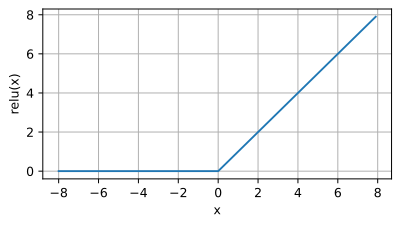
\includegraphics[width=0.7]{../imgs/ReLU.eps}
    \end{enumerate}


\end{document}